\chapter{Technologies} \label{ch:technologies}

\section{Docker}
When discussing containers, Docker cannot be left out of the discussion. Docker is an open-source platform designed to automate the creation, deployment, scaling, and management of containerized applications. It is, by far, the most widely adopted tool for containerization. Docker allows the packaging of applications and their dependencies into lightweight and easily portable containers that can be deployed consistently across a wide range of environments. This portability ensures that applications behave identically, whether running on a developer's laptop, a staging environment, or a production server.

To provision containers, Docker uses images. Docker images are read-only templates used to create containers, similar to .iso files for virtual machines, but are more lightweight and versatile. Docker images bundle everything an application needs to run, including the operating system, application code, dependencies, libraries, and configuration metadata. The metadata often includes the entry point script, a set of commands executed when the container is instantiated.

An important feature of Docker images is their layered architecture. Each layer represents a distinct change, such as adding a file, installing a package, or modifying a configuration. This layered design allows developers to build images on top of existing ones, significantly reducing build times, image sizes, and data transfer requirements.

The runtime environment responsible for building, running, and managing containers is the Docker Engine, and it consists of three main components. The first is the Docker Daemon, a background service responsible for managing Docker objects, such as containers, images, volumes, and networks. Next is the Docker Command-Line Interface (CLI), which provides a way to interact with Docker through terminal commands. Finally, the REST API enables programmatic access to Docker's functionalities.

Docker images are created using Dockerfiles, which act as blueprints for the image creation process. A Dockerfile contains step-by-step instructions for building an image, including the base image, commands to configure the environment, install dependencies, and metadata such as port configurations and the entrypoint script. This declarative approach ensures reproducibility, as anyone with the Dockerfile can recreate the same image, ensuring consistency across teams.

Since images are meant to be portable and used over multiple environments, remote registries to store and fetch images from are crucial. Docker Hub is a free, widely used registry provided by the wider Docker ecosystem.

Hand in hand with containers, Docker enables the creation and management of other resources, critical for smooth operation. Volumes are a mechanism for persisting data generated and used by containers. Unlike ephemeral container storage, volumes ensure data remains intact even after container deletion. Docker also creates networks, enabling container inter-connectivity and communication between containers and the outside world.

For handling deployments of multiple containers in a programmatic way, Docker Compose can be utilized. Docker Compose is a tool that utilizes simple YAML files to manage multi-container deployments or applications by defining services, networks, and volumes required. This approach reduces complexity and enhances reproducibility, making it easier to manage applications with multiple inter-connected components.

Finally, Docker provides a native container orchestration platform, Docker Swarm, but on a production level, it is outclassed by other, more robust and feature-rich solutions, such as bare-metal Kubernetes or cloud Kubernetes services like Amazon Elastic Kubernetes Service (EKS) and Google Kubernetes Engine (GKE) that offer seamless integration and scalability.\cite{containers_docker}


\begin{figure}[!h]
    \graphicspath{ {./diagrams/} }
    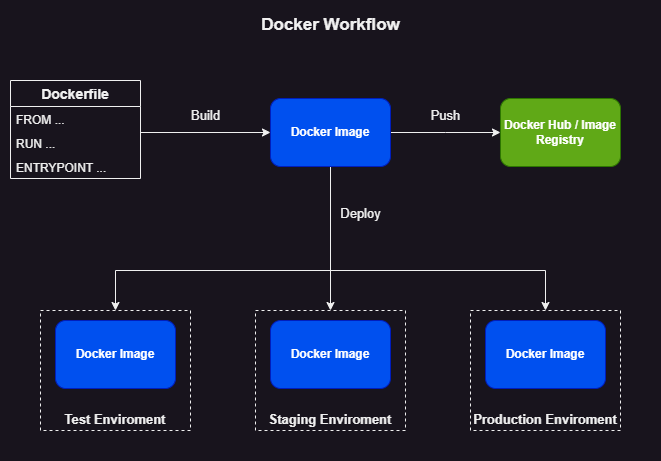
\includegraphics[scale=0.6]{docker_wf.png}
    \centering
    \caption{Docker Workflow}
    \label{fig:docker_wf}
\end{figure}

\section{Prometheus}
Prometheus is an open-source monitoring and alerting toolkit designed to provide flexible, reliable, and robust monitoring for any type of numerical data. It is considered a foundational tool for observability and a key component of modern monitoring stacks. Prometheus excels in collecting, storing, and querying time-series metrics, making it an ideal choice for monitoring infrastructure, applications, and containerized environments.

Prometheus collects and stores metrics as time-series data. Every metric is stored alongside a timestamp, allowing users to track and analyze changes over time. This feature is invaluable for identifying trends, diagnosing performance bottlenecks, and understanding long-term system behavior. Prometheus operates using a pull-based model, periodically scraping selected targets for metrics. This model ensures efficiency by fetching only the required data and enhances security by not requiring external systems to push data directly into Prometheus.

Metrics from various sources are exposed through services called Exporters, which transform raw data into a Prometheus-readable format. Prometheus includes a large ecosystem of pre-built exporters for common targets such as hardware systems, databases, and cloud platforms. Additionally, creating custom exporters is straightforward, making Prometheus highly adaptable to diverse use cases.

For retrieving, filtering, and manipulating time-series data, Prometheus Query Language (PromQL) is used. PromQL allows users to extract meaningful insights, create advanced visualizations, and define custom alerting rules. Prometheus also integrates seamlessly with Alertmanager, a companion tool for managing alerts. Users can define alerting rules based on PromQL expressions to trigger notifications when specific conditions, such as threshold breaches or anomalies, are met. Alertmanager routes these alerts to appropriate channels, such as email, Slack, or webhooks.

For short-lived jobs that may terminate before Prometheus can scrape their metrics, the PushGateway provides a solution. This intermediary gateway allows these jobs to push metrics at creation time, ensuring no data loss. Prometheus also supports Service Discovery, enabling automatic detection of scrape targets in dynamic environments like Kubernetes. This eliminates the need for manual configuration, making it ideal for large-scale, constantly changing systems.

Prometheus employs a highly optimized, custom-built database for storing time-series data. This database supports fine-grained retention policies, allowing users to define which metrics to retain and for how long, thereby optimizing storage usage. Prometheus further enhances usability with its ability to label metrics using key-value pairs. These labels provide additional context and facilitate filtering and aggregation, enabling multidimensional analysis of metrics.

Although Prometheus offers basic visualization capabilities, it integrates natively with Grafana, the industry-leading visualization platform. This integration allows users to build interactive, feature-rich dashboards. While Prometheus is optimized for metrics collection, it is not suitable for other types of data, such as logs. To fill these voids from Prometheus, tools like Loki are often used to handle log data, creating a comprehensive observability stack.\cite{Jani2024-mg,Pragathi2024-fa}



\section{Grafana}
Usually, when utilizing Prometheus to gather metrics, Grafana is employed as the visualization tool of choice. Grafana is an open-source platform for monitoring and observability, designed to enable users to visualize, query, and analyze data from an extensive range of data sources. By transforming raw metrics into actionable insights, Grafana facilitates the creation of complex, interactive dashboards, making it an essential component of most modern monitoring and observability implementations.

These dashboards are highly customizable, combining a diverse variety of visualizations, such as line graphs, heatmaps, gauges, tables, and single-stat panels. This flexibility allows teams to represent various types of information, including historical data, real-time system statuses, and long-term trends, in a visually appealing and intuitive manner.

Grafana supports integration with a broad array of data sources, including Prometheus, Loki, PostgreSQL, MySQL, and cloud services. Its ability to query multiple sources simultaneously enables advanced, multifaceted analyses, where data from diverse systems can be combined and manipulated for deeper insights.

Grafana also has support for variable creation, which allows users to dynamically assign values from the sourced data. This capability enables the construction of dynamic dashboards with parameterized views that adapt to different environments, datasets, or conditions without requiring additional customization. Such dynamic behavior unlocks templating, where reusable dashboards can be developed, significantly enhancing efficiency and consistency across monitoring setups.

Grafana excels at centralizing observability, providing a unified view of the health and performance of systems, services, and applications. Its real-time visualizations empower teams to detect and address issues as they emerge, enabling faster response times and minimizing downtime.

At the same time, the ability to chart and analyze historical data enables the identification of recurring trends and the prediction of potential problems, thus allowing the implementation of proactive measures to mitigate risks.

Lastly, Grafana offers alerting capabilities, same as Prometheus with Alertmanager, that can push notifications on various channels when a set of conditions is met\cite{grafana, promandgraf}.

\begin{figure}[!h]
    \graphicspath{ {./diagrams/} }
    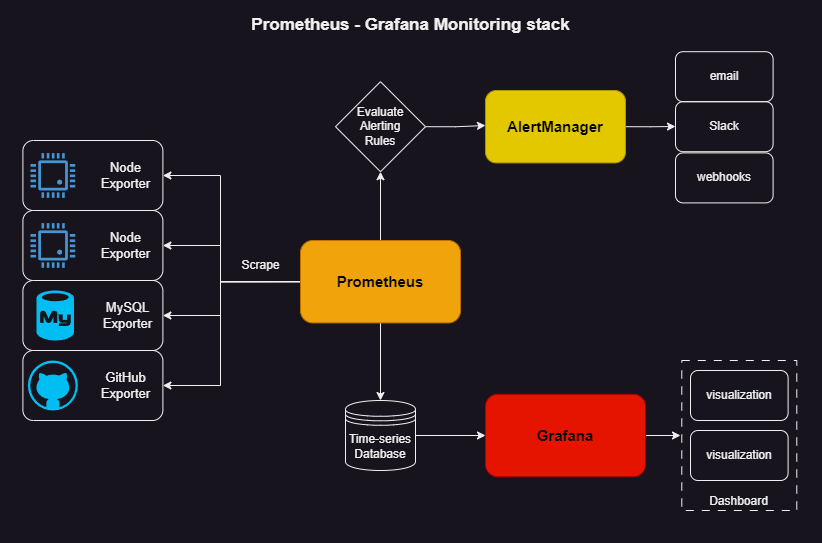
\includegraphics[scale=0.55]{prom-graf.png}
    \centering
    \caption{Prometheus-Grafana Monitoring stack}
    \label{fig:prom_graf}
\end{figure}

\section{Message Queuing Telemetry Transport (MQTT)}
Message Queuing Telemetry Transport (MQTT) is a lightweight, publish/subscribe model messaging protocol specifically designed for devices with limited computational resources and unreliable, low-bandwidth networks. Its efficiency and reliability make it a standard choice for IoT device communication and similar constrained environments.

At its core, MQTT operates using the publish/subscribe model, a decoupled communication architecture where publishers (senders) and subscribers (receivers) exchange messages through a central broker. The MQTT broker serves as the backend system responsible for managing message coordination between clients. Its key responsibilities include receiving and filtering messages, identifying clients subscribed to specific topics, and forwarding messages to those subscribers. Popular MQTT brokers are EMQX, HiveMQ and Mosquitto. Mosquitto was preferred in this implementation for it's lightweight nature, which fits well in a microservice approach.

In typical communication, MQTT clients (which can act as publishers, subscribers, or both) establish a connection with the broker using an MQTT connection. The broker confirms the connection, ensuring both entities are ready to exchange messages. MQTT requires a TCP/IP stack on both clients and brokers for communication, and clients never connect directly with each other but only with the broker. Once connected, the client can either publish messages, subscribe to specific messages, or do both. The broker filters incoming messages using topics, which are structured hierarchically, similar to folder directories in a filesystem. The broker only sends messages to subscribers from the topics they have explicitly subscribed to.

The MQTT protocol is widely regarded as a standard for IoT data transmission and for good reason. Firstly, it requires minimal hardware resources, so it can even be used by small battery-powered microcontrollers. MQTT control messages and MQTT message headers are quite small, reducing network overhead and ensuring efficient use of bandwidth. MQTT has build-in features like quick device reconnections and quality-of-service (QoS) levels, which ensure reliable message delivery even on the unreliable, low-bandwidth and high latency cellular networks IoT devices usually operate on. The decouple nature of MQTT, combined with the low bandwidth requirements allows it to easily handle large number of clients, making it very scalable. 

Despite its many strengths, MQTT does have a few limitations. The broker acts as the central node, and subsequently as a single point of failure, so any disruption or failure of the broker results in a complete communication breakdown. This risk can be mitigated through high-availability setups. Also the maximum payload is 256MB and large payloads can impact performance, however in an IoT scenario such large payloads are uncommon. Lastly, MQTT lacks native encryption but modern authentication protocols such as OAuth and TLS can be easily integrated, to enhance security\cite{mqtt}.

\begin{figure}[!h]
    \graphicspath{ {./diagrams/} }
    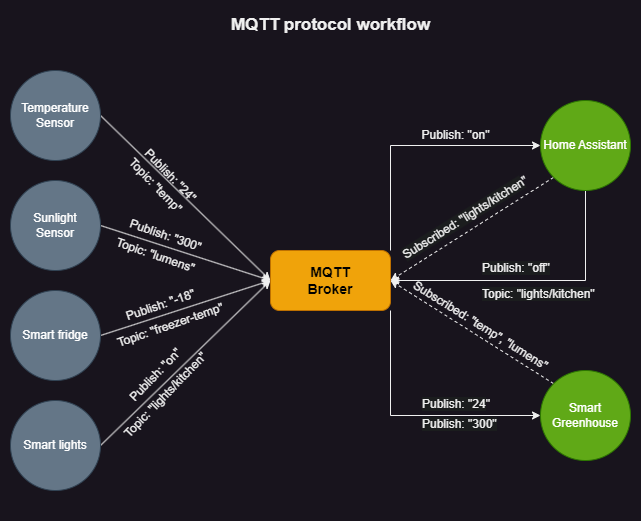
\includegraphics[scale=0.7]{mqtt.png}
    \centering
    \caption{MQTT protocol workflow}
    \label{fig:mqtt}
\end{figure}